%Testbeds
\chapter{Testbeds}
Included here is a brief description of the data sources that will be used for this work.

%Brown Hall
\section{University Buildings}
\begin{figure}[ht]
\begin{center}
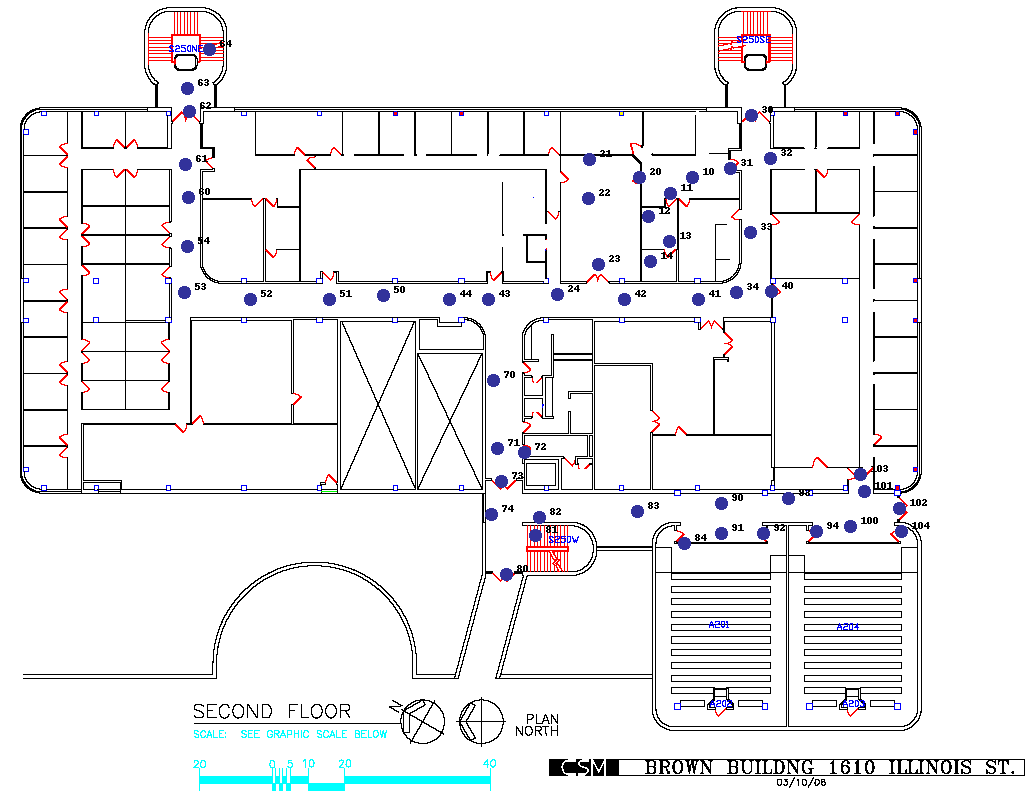
\includegraphics[width=0.6\textwidth]{brown_motes.png}
\end{center}
\caption{Mote locations on the second floor of the Colorado School of Mines Brown Building.}
\label{fig:brown_motes}
\end{figure}

Infrared motion counts from a class room building at the Colorado School of Mines.  Simple infrared motion sensors were placed throughout the floor and were polled for motion data every second.  This data has a predictable time of day model based on class times with Monday, Wednesday and Friday following a different schedule than Tuesday and Thursday.

Additionally we plan to have access to the Colorado School of Mines Center for Technology and Learning Media building's camera data.  Camera data will be converted into motion data describing the number of people moving in any direction at a given time.  This building serves as a class room building, computing center, and student congregation area due to the presence of an Einstein's bagels.  

%Colorado Department of Transportation
\section{Denver Traffic}
\begin{figure}[ht]
\begin{center}
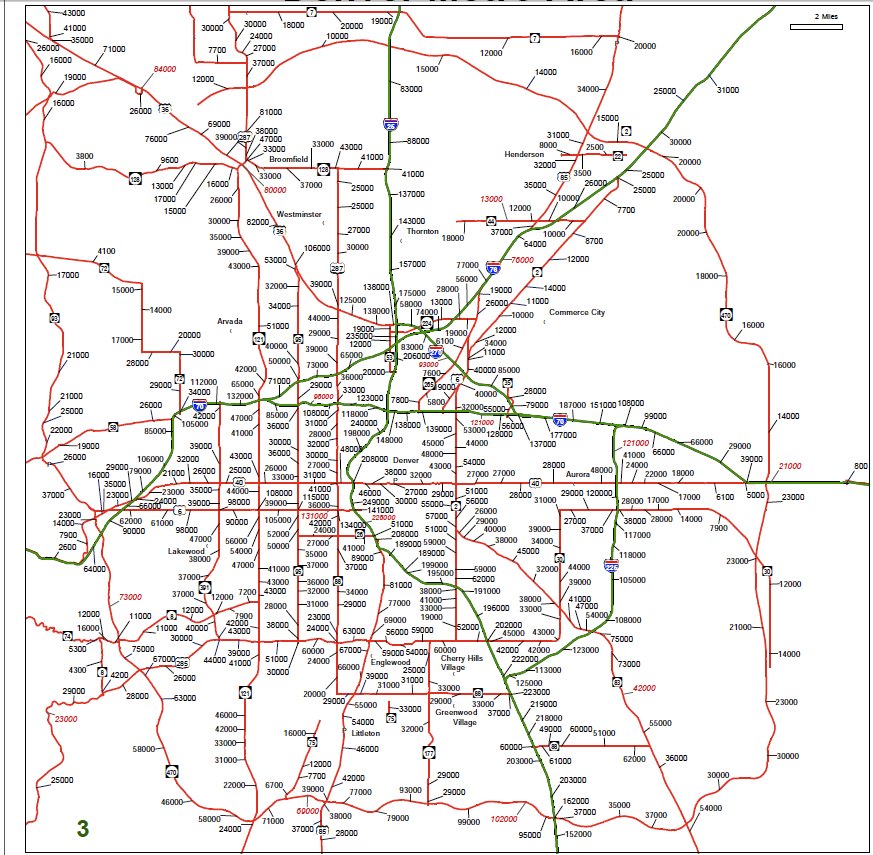
\includegraphics[width=0.6\textwidth]{traffic_sensors.png}
\end{center}
\caption{Traffic count sensor locations near the city of Denver.}
\label{fig:denver_sensors}
\end{figure}

Traffic count sensors from various locations near the city of Denver.  Count data is aggregated per hour for each direction of traffic at every sensor location.  This data is highly repetitive as Monday through Thursday have approximately the same daily traffic patterns.  Friday behaves much like the rest of the weekdays with the differences being that evening rush hour happens about an hour earlier and their is an increase in night activity.  

%Simulator
\section{Simulator}
As another way to produce building motion behavior a simulator has been created.  It is used primarily to create specific test runs which are used to give a better indicator of the performance of our methods.

The simulator creates a model of background information by mimicking typical single person activities such as occasional travel to the bathroom, vending machine, water cooler, etc.  This background information is present throughout the simulation however it does not have to be constant.  The possible locations and function that determines frequency of travel can be changed at any time.  

On top of this background model, the simulator mimics various types of activities.  Sample activities include meetings, lunch time exodus, or fire drills.  For each of these activities, the number of people present along with functions that determine probability of arrival time (which includes the possibility of being late) and leave times are possible.  These parameters allow for multiple types of meetings to be simulated.  

One additional but important feature of the simulation is that it allows for sensors to have any type of sensing function.  The simulator can mimic almost any type of sensor instead of simply radial infrared sensors.